\subsubsection{x86}

\index{x86!\Instructions!LOOP}
\RU{Для организации циклов, в архитектуре x86 есть старая инструкция \LOOP, 
она проверяет значение регистра \ECX и если оно не $0$, делает \glslink{decrement}{декремент} \ECX 
и переход по метке указанной в операнде. 
Возможно, эта инструкция не слишком удобная, поэтому я не видел современных компиляторов, 
которые использовали бы её. Так что, если вы видите где-то \LOOP, то это, с большой вероятностью, 
вручную написанный код на ассемблере.}
\EN{There is a special \LOOP instruction in x86 instruction set, it is checking value in the \ECX register and 
if it is not $0$, do \ECX \gls{decrement}
and pass control flow to the label mentioned in the \LOOP operand. 
Probably, this instruction is not very convenient, so, I did not ever see any modern compiler emit it automatically.
So, if you see the instruction somewhere in code, it is most likely this is manually written piece 
of assembly code.}\\
\\
\RU{Обычно, циклы на \CCpp создаются при помощи \TT{for()}, \TT{while()}, \TT{do/while()}.}
\EN{In \CCpp loops are usually constructed using \TT{for()}, \TT{while()}, \TT{do/while()} statements.}

\RU{Начнем с}\EN{Let's start with} \TT{for()}.
\index{\CLanguageElements!for}

\RU{Это выражение описывает инициализацию, условие, что делать после каждой итерации
(\glslink{increment}{инкремент}/\glslink{decrement}{декремент})
и тело цикла.}
\EN{This statement defines loop initialization (set loop counter to initial value), 
loop condition (is counter is bigger than a limit?), what is done at each iteration (\gls{increment}/\gls{decrement})
and of course loop body.}

\lstinputlisting{patterns/09_loops/simple/loops_1_\LANG.c}

\RU{Примерно так же, генерируемый код и будет состоять из этих четырех частей.}
\EN{So, generated code will be consisted of four parts as well.}

\RU{Возьмем пример}\EN{Let's start with simple example}:

\lstinputlisting[label=loops_src]{patterns/09_loops/simple/loops_2.c}

\RU{Имеем в итоге}\EN{Result} (MSVC 2010):

\lstinputlisting[caption=MSVC 2010]{patterns/09_loops/simple/1_MSVC_\LANG.asm}

\RU{В принципе, ничего необычного.}\EN{Nothing very special, as we see.}

\RU{GCC 4.4.1 выдает примерно такой же код, с небольшой разницей:}
\EN{GCC 4.4.1 emits almost the same code, with one subtle difference:}

\lstinputlisting[caption=GCC 4.4.1]{patterns/09_loops/simple/1_GCC_\LANG.asm}

\RU{Интересно становится, если скомпилируем этот же код при помощи MSVC 2010 с включенной оптимизацией}
\EN{Now let's see what we will get if optimization is turned on} (\Ox):

\lstinputlisting[caption=\Optimizing MSVC]{patterns/09_loops/simple/1_MSVC_Ox.asm}

\RU{Здесь происходит следующее: переменную $i$ компилятор не выделяет в локальном стеке, 
а выделяет целый регистр под нее: \ESI. 
Это возможно для маленьких функций, где мало локальных переменных.}
\EN{What is going on here is: space for the $i$ variable is not allocated in local stack anymore,
but individual register is allocated for it: the \ESI.
This is possible in such small functions where not so many local variables are present.}

\RU{В принципе, все то же самое, только теперь одна важная особенность: 
\ttf не должна менять значение \ESI. 
Наш компилятор уверен в этом, а если бы и была необходимость использовать регистр \ESI в функции \ttf, 
то её значение сохранялось бы в стеке. Примерно так же, как и в нашем листинге: 
обратите внимание на \TT{PUSH ESI/POP ESI} в начале и конце функции.}
\EN{One very important property is the \ttf function must not change the value in the \ESI.
Our compiler is sure here. 
And if compiler decided to use the \ESI register in \ttf too, its value would be saved then 
at the \ttf function's prologue and restored at the \ttf function's epilogue.
Almost like in our listing: please note \TT{PUSH ESI/POP ESI}
at the function begin and end.}

\RU{Попробуем GCC 4.4.1 с максимальной оптимизацией (\Othree):}
\EN{Let's try GCC 4.4.1 with maximal optimization turned on (\Othree option):}

\lstinputlisting[caption=\Optimizing GCC 4.4.1]{patterns/09_loops/simple/1_GCC_O3.asm}

\index{Loop unwinding}
\RU{Однако, GCC просто \IT{развернул} цикл\footnote{\gls{loop unwinding} в англоязычной литературе}.}
\EN{Huh, GCC just unwind our loop.}

\RU{Делается это в тех случаях, когда итераций не слишком много, как в нашем примере, 
и можно немного сэкономить время, убрав все инструкции, обеспечивающие цикл. 
В качестве обратной стороны медали, размер кода увеличился.}
\EN{\Gls{loop unwinding} has advantage in these cases when there is not so much iterations and 
we could cut some execution speed by removing all loop supporting instructions. 
On the other side, resulting code is obviously larger.}
% FIXME но в наше время это уже не нужно

\RU{OK, увеличим максимальное значение $i$ в цикле до $100$ и попробуем снова. GCC выдаст подобное:}
\EN{OK, let's increase maximal value of the $i$ variable to $100$ and try again. GCC will do:}

\lstinputlisting[caption=GCC]{patterns/09_loops/simple/2_GCC_\LANG.asm}

\RU{Это уже похоже на то что сделал MSVC 2010 в режиме оптимизации (\Ox). 
За исключением того, что под переменную $i$ будет выделен регистр \EBX.}
\EN{It is quite similar to what MSVC 2010 with optimization (\Ox) produce. 
With the exception the \EBX register will be fixed to the $i$ variable.}
\RU{GCC уверен, что этот регистр не будет 
модифицироваться внутри \ttf, а если вдруг это и придётся там сделать, то его значение будет сохранено 
в начале функции, прямо как в \main здесь.}
\EN{GCC is sure this register will not be modified inside of the \ttf function, 
and if it will, it will be saved at the function prologue and restored at epilogue, 
just like here in the \main function.}

\ifdefined\IncludeOlly
\clearpage
\subsubsection{x86: \olly}
\index{\olly}

\RU{Скомпилируем наш пример в}\EN{Let's compile our example in} MSVC 2010 \RU{с}\EN{with} \Ox \AndENRU \Obzero 
\RU{и загрузим в}\EN{options and load it into} \olly.

\RU{Оказывается}\EN{It seems}, \olly \RU{может обнаруживать простые циклы и показывать их в квадратных скобках, 
для удобства}\EN{is able to detect simple loops and show them in square brackets, for convenience}:

\begin{figure}[H]
\centering
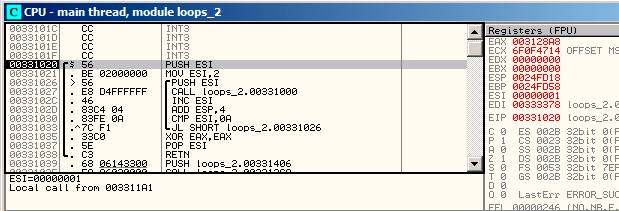
\includegraphics[scale=\FigScale]{patterns/09_loops/simple/olly1.png}
\caption{\olly: \RU{начало \main}\EN{\main begin}}
\label{fig:loops_olly_1}
\end{figure}

\RU{Трассируя}\EN{By tracing} (F8 (\stepover)) \RU{мы видим как}\EN{we see how} \ESI \RU{увеличивается на 1}
\EN{\glslink{increment}{incrementing}}.
\RU{Например, здесь}\EN{Here, for instance,} $ESI=i=6$:

\begin{figure}[H]
\centering
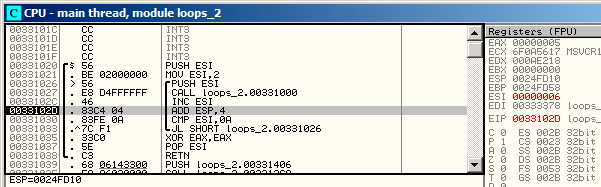
\includegraphics[scale=\FigScale]{patterns/09_loops/simple/olly2.png}
\caption{\olly: \RU{тело цикла только что отработало с}\EN{loop body just executed with} $i=6$}
\label{fig:loops_olly_2}
\end{figure}

$9$ \RU{это последнее значение цикла}\EN{is a last loop value}.
\RU{Поэтому}\EN{That's why} \JL \RU{после \glslink{increment}{инкремента} не срабатывает и ф-ция заканчивается}
\EN{will not trigger after \gls{increment}, and function is finishing}:

\begin{figure}[H]
\centering
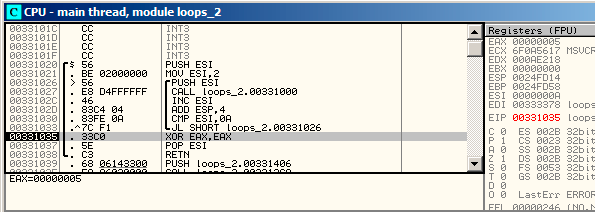
\includegraphics[scale=\FigScale]{patterns/09_loops/simple/olly3.png}
\caption{\olly: $ESI=10$, \RU{конец цикла}\EN{loop end}}
\label{fig:loops_olly_3}
\end{figure}

\subsubsection{x86: tracer}
\index{tracer}

\RU{Как видно, трассировать вручную цикл в отладчике это не очень удобно}\EN{As we might see, it is not very
convenient to trace in debugger manually}.
\RU{Это одна из причин, почему я писал}\EN{That's one of the reasons I wrote} \tracer \RU{для себя}
\EN{for myself}.

\RU{Я открываю скомпилированный пример в}\EN{I open compiled example in} \IDA, 
\RU{нахожу там адрес инструкции}\EN{I find the address of the instruction} \TT{PUSH ESI}
(\RU{передающей единственный аргумент в}\EN{passing sole argument into} \ttf) 
\RU{а это}\EN{and this is} \TT{0x401026} \RU{у меня и запускаю}\EN{for me and I run} \tracer:

\begin{lstlisting}
tracer.exe -l:loops_2.exe bpx=loops_2.exe!0x00401026
\end{lstlisting}

\RU{Опция }\TT{BPX} \RU{просто ставит брякпойнт по адресу и затем будет выдавать состояние регистров}
\EN{just sets breakpoint at address and then will print registers state}.

\RU{В}\EN{In the} \TT{tracer.log} \RU{после запуска я вижу следующее}\EN{I see after running}:

\lstinputlisting{patterns/09_loops/simple/tracer.log}

\RU{Видно как значение}\EN{We see how value of} \ESI \RU{последовательно изменяется от 2 до 9}
\EN{register is changed from 2 to 9}.

\RU{И дажее более того, в \tracer можно собирать значения регистров по всем адресам внутри ф-ции}
\EN{Even more than that, \tracer can collect register values on all addresses within function}.
\RU{Там это называется}\EN{This is called} \IT{trace}\EN{ there}.
\RU{Каждая инструкция трассируется, значения самых интересных регистров запоминаются}\EN{Each instruction
is being traced, all interesting register values are noticed and collected}.
\RU{Затем генерируется .idc-скрипт для \IDA, который добавляет комментарии.}
\EN{\IDA .idc-script is generated then.}
\RU{Итак, в}\EN{So, in the} \IDA \RU{я узнал что адрес}\EN{I've learned that} \main \RU{это}\EN{function address
is} \TT{0x00401020} \RU{и запускаю}\EN{and I run}:

\begin{lstlisting}
tracer.exe -l:loops_2.exe bpf=loops_2.exe!0x00401020,trace:cc
\end{lstlisting}

\TT{BPF} \RU{означает установить брякпойнт на ф-ции}\EN{mean set breakpoint on function}.

\RU{Получаю в итоге скрипты}\EN{As a result, I have got} \TT{loops\_2.exe.idc} \AndENRU 
\TT{loops\_2.exe\_clear.idc}\EN{ scripts}.

\clearpage
\RU{Загружаю}\EN{I'm loading} \TT{loops\_2.exe.idc} \RU{в}\EN{into} \IDA \RU{и увижу следующее}\EN{and I see}:

\begin{figure}[H]
\centering
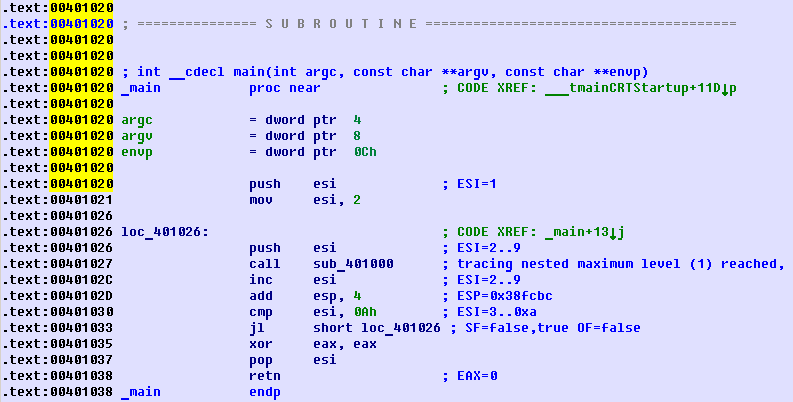
\includegraphics[scale=\FigScale]{patterns/09_loops/simple/IDA_tracer_cc.png}
\caption{\IDA \RU{с загруженным .idc-скриптом}\EN{with .idc-script loaded}}
\label{fig:loops_IDA_tracer}
\end{figure}

\RU{Видно что}\EN{We see that} \ESI \RU{бывает от 2 до 9 в начале тела цикла, но после 
\glslink{increment}{инкремента} он в пределах [3..0xA]}\EN{can be from 2 to 9 at the begin of loop body,
but from 3 to 0xA (10) after increment}.
\RU{Видно также что ф-ция}\EN{We can also see that} \main \RU{заканчивается с 0 в}\EN{is finishing with 0 in} \EAX.

\tracer \RU{также генерирует}\EN{also generates} \TT{loops\_2.exe.txt}, 
\RU{содержащий адреса инструкций, сколько раз была исполнена
каждая и значения регистров}\EN{containing information about how many times each instruction was executed and
register values}:

\lstinputlisting[caption=loops\_2.exe.txt]{patterns/09_loops/simple/loops_2.exe.txt}
\index{\GrepUsage}
\RU{Так можно использовать grep}\EN{grep can be used here}.

\fi
